% !TEX encoding = UTF-8 Unicode

\documentclass[spanish,xcolor=table,svgnames]{beamer}
\definecolor{mediumpurple4}{rgb}{0.36,0.28,0.55}
%colores coporativos
\definecolor{naranja}{rgb}{0.86,0.42,0.06}
\definecolor{gris}{rgb}{0.41,0.41,0.41}
\definecolor{azul}{rgb}{0.06,0.31,0.55}
\definecolor{rojo}{rgb}{1,0,0}
\usecolortheme[named=azul]{structure}

\mode<presentation>
{

  \usetheme{Warsaw}
%\useoutertheme{infolines}
  \setbeamercovered{transparent}
  \setbeamertemplate{navigation symbols}{}
}
\usepackage{listings}
\usepackage{color}
\definecolor{gray97}{gray}{.97}
\definecolor{gray75}{gray}{.75}
\definecolor{gray45}{gray}{.45}
\usepackage{listings}
\lstset{ frame=Ltb,
     framerule=0pt,
     aboveskip=0.5cm,
     framextopmargin=3pt,
     framexbottommargin=3pt,
     framexleftmargin=0.4cm,
     framesep=0pt,
     rulesep=.4pt,
     backgroundcolor=\color{gray97},
     rulesepcolor=\color{black},
     %
     stringstyle=\ttfamily,
     showstringspaces = false,
     basicstyle=\small\ttfamily,
     commentstyle=\color{blue},
     keywordstyle=\bfseries,
     %
     numbers=left,
     numbersep=15pt,
     numberstyle=\tiny,
     numberfirstline = false,
     breaklines=true,
   }
 
% minimizar fragmentado de listados
\lstnewenvironment{listing}[1][]
   {\lstset{#1}\pagebreak[0]}{\pagebreak[0]}
 \lstdefinestyle{consola}
   {basicstyle=\scriptsize\bf\ttfamily,
    backgroundcolor=\color{gray75},
   }
\lstdefinestyle{consola}
   {basicstyle=\scriptsize\bf\ttfamily,
    backgroundcolor=\color{gray75},
   }

\lstdefinestyle{XML}
   {language=XML,
   }

\usepackage[spanish]{babel}
\usepackage[utf8]{inputenc}
\usepackage{charter}
\usepackage[T1]{fontenc}
\usepackage{fancyvrb}
\usepackage{tikz}
%\usepackage{microtype}
\usepackage{xspace}
\usepackage{ctable}
\usepackage{alltt,multicol}

\newcommand{\reduce}{\fontsize{8}{9}\selectfont}
%\usetikzlibrary{chains,positioning,decorations.pathreplacing,fit,scopes}

\title[Gestión de Centro de Mejora del Rendimiento y la Salud]{Gestión de Centro de Mejora del Rendimiento y la Salud}
\author[Jesús Soriano Candón]{Jesús Soriano Candón\\Tutora: Lorena Gutiérrez Madroñal}
\institute[UCA]{Ingenierí­a Informática}
\date{15 de diciembre de 2017}

\DefineVerbatimEnvironment{vrbwithcmd}{Verbatim}{commandchars=+(),fontsize=\small}

\begin{document}

\begin{frame}
  \titlepage
  \begin{figure}
	
\includegraphics[width=0.2\textheight]{logo_uca} 
  \end{figure}
\end{frame}

\frame{\frametitle{͍ndice}\tableofcontents}

%%%%%%%%%%%%%%%%%%%%%%%%%%%%%%%%%
\section{Introducción}
\begin{frame}{Introducción}
    \tableofcontents[currentsection]
\end{frame}

\subsection*{Motivación}
\begin{frame}{Motivación}
  \begin{columns}[onlytextwidth]
    \begin{column}{0.5\textwidth}
      \begin{block}{Motivación del proyecto}
        \begin{itemize}
          \item CoreSport, centro de mejora del rendimiento y la salud.
          \item Necesidad de un sistema telemático de gestión.
          \item Facilitar la gestión a administradores y usuarios.
          \item Necesidad de web pública.
        \end{itemize}
      \end{block}
    \end{column}
    \begin{column}{0.5\textwidth}
      \centering
      \begin{figure}[H]
        \begin{center}
        
\includegraphics[width=0.9\textwidth]{img/coresport.png}
        \end{center}
        \label{fig:logo-coresport}
      \end{figure}
    \end{column}
€‹  \end{columns}
\end{frame}


\subsection*{Alcance}
\begin{frame}{Alcance}
\begin{block}{Objetivo}
Proporcionar una herramienta de gestión de las necesidades del centro para los administradores y de actividades y citas para usuarios. \\
Además de la realización de la página web del centro.
\end{block}
\end{frame}



%%%%%%%%%%%%%%%%%%%%%%%%%%%%%%%%%
\section{Planificación}
\frame{\frametitle{Planificación}\tableofcontents[currentsection]}

\subsection*{Metodologí­a}
\begin{frame}{Metodologí­a}
    \begin{center}
    Modelo Incremental
    \begin{figure}[H]
      \begin{center}
          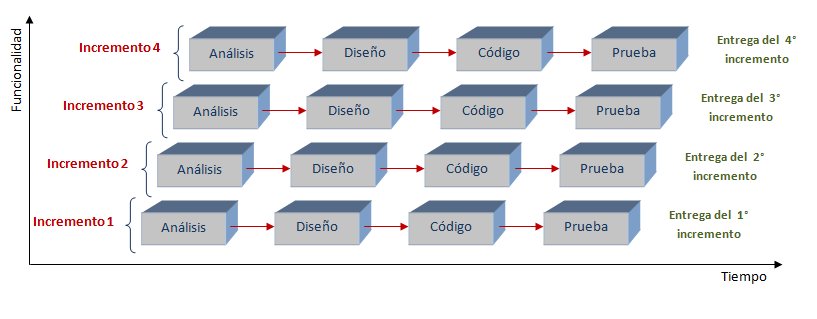
\includegraphics[width=\textwidth]{img/modelo-incremental.png}
      \end{center}
      \label{fig:modelo-incremental}
    \end{figure}
  \end{center}
\end{frame}

\subsection*{Calendario}
\begin{frame}{Calendario}
  \begin{center}
    \begin{figure}[H]
      \begin{center}
          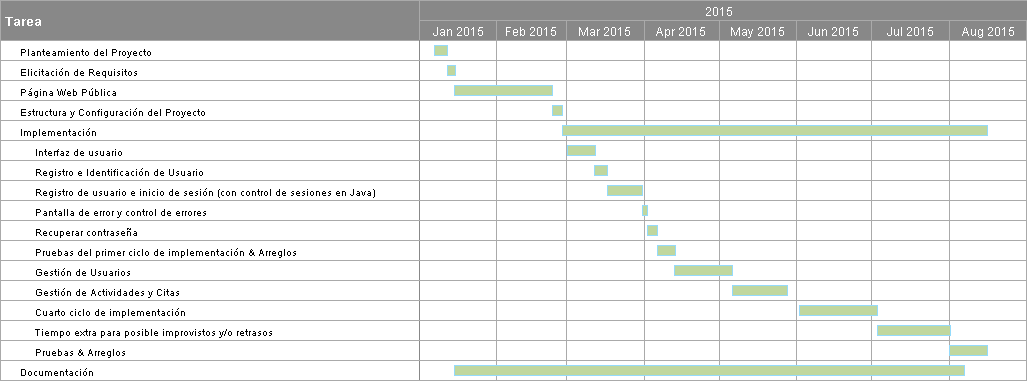
\includegraphics[width=1.0\textwidth]{img/planificacion-gantt.png}
      \end{center}
      \caption{Diagrama de Gantt con tiempos estimados}
      \label{fig:gantt}
    \end{figure}
  \end{center}
\end{frame}


%%%%%%%%%%%%%%%%%%%%%%%%%%%%%%%
\section{Desarrollo del Proyecto}
\frame{\frametitle{Desarrollo del proyecto}\tableofcontents[currentsection]}

\subsection*{Requisitos}
\begin{frame}{Requisitos Funcionales}
  \begin{block}{Requisitos Funcionales}
    \begin{column}{0.5\textwidth}
  \begin{itemize}
    \item Selector de idiomas.
    \item Gestión de datos de usuarios y contraseñas.
    \item Gestión de clases, citas y otros servicios.
    \item Calendario de actividades y citas.
  \end{itemize}
    \end{column}
    \begin{column}{0.5\textwidth}
  \begin{itemize}
    \item Notificaciones.
    \item Registro de operaciones.
    \item Comunicación interna.
    \item *Gestión de usuarios.
    \item *Gestión completa de servicios: Actividades, citas y archivos.
  \end{itemize}
    \end{column}
  \end{block}
  * Requisitos funcionales para administradores.
\end{frame}

\begin{frame}{Requisitos no Funcionales}
  \begin{block}{Requisitos no Funcionales}
  \begin{itemize}
    \item Disponibilidad.
  \begin{itemize}
    \item Adaptabilidad.
  \end{itemize}
    \item Fiabilidad.
    \item Internacionalización.
    \item Usabilidad.
    \item Mantenibilidad.
  \end{itemize}
  \end{block}
\end{frame}



\subsection*{Análisis}
\begin{frame}{Model Conceptual}
  \begin{figure}[H]
    \begin{center}
        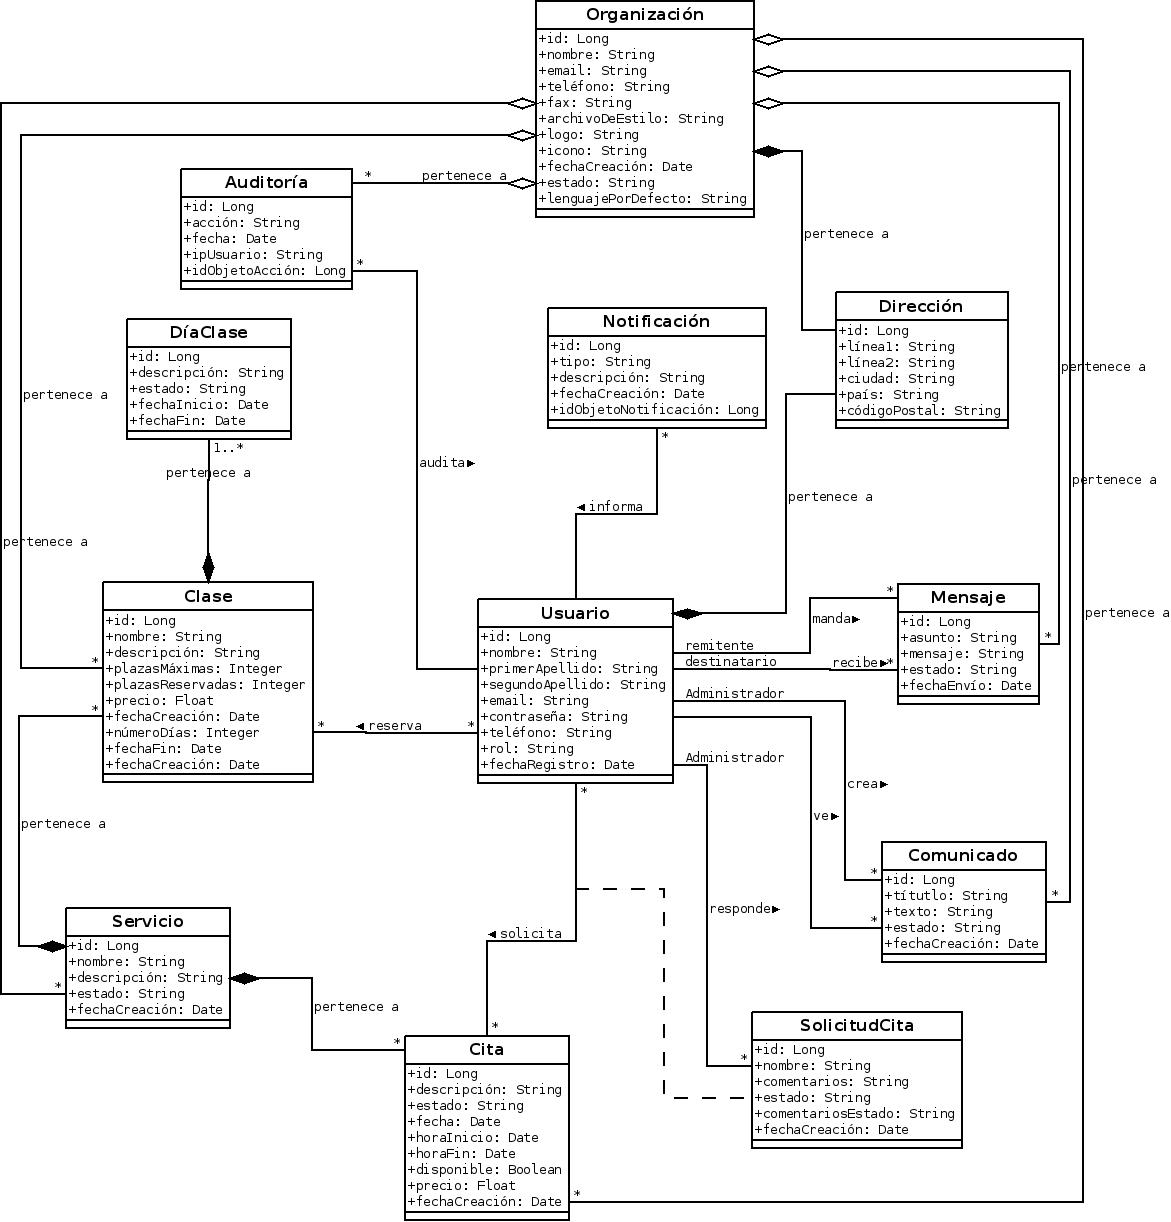
\includegraphics[width=0.6\textwidth]{img/modelo-conceptual.jpeg}
    \end{center}
    \label{fig:conceptual}
\end{figure}
\end{frame}


\subsection*{Diseño}
\begin{frame}{Diseño de Interfaz de Usuario}
  \begin{figure}[H]
    \begin{center}
        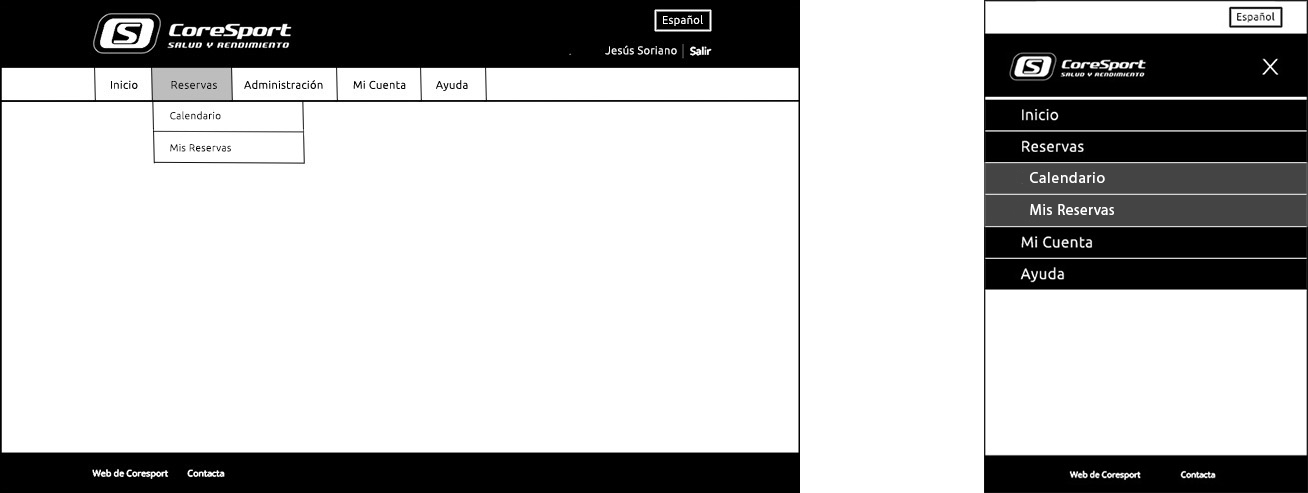
\includegraphics[width=0.7\textwidth]{img/comparativa-interfaces.png}
    \end{center}
      \caption{Diseño adaptable (responsive)}
    \label{fig:responsive}
\end{figure}
\end{frame}

\begin{frame}{Diseño de Interfaz de Usuario}
  \begin{figure}[H]
    \begin{center}
      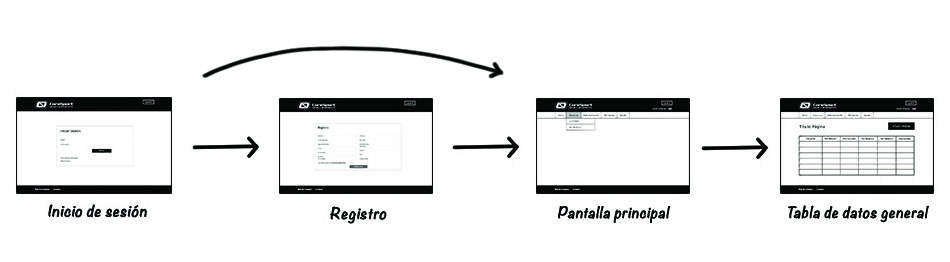
\includegraphics[width=1.0\textwidth]{img/navegacion.jpg}
    \end{center}
      \caption{Navegación}
    \label{fig:navegacion}
\end{figure}
\end{frame}





\subsection*{Implementación}

\begin{frame}{Entorno Tecnológico}
  \begin{figure}[H]
    \begin{center}
        
\includegraphics[width=0.75\textwidth]{img/logos-combinados.jpg}
    \end{center}
    \label{fig:tecnologias}
  \end{figure}
\end{frame}

\begin{frame}{Entorno Tecnológico}
  \begin{figure}[H]
    \begin{center}
        
\includegraphics[width=0.75\textwidth]{img/logos-combinados-java.jpg}
    \end{center}
    \label{fig:tecnologias-java}
  \end{figure}
\end{frame}

\begin{frame}{Entorno Tecnológico}
  \begin{figure}[H]
    \begin{center}
        
\includegraphics[width=0.75\textwidth]{img/logos-combinados-postgresql.jpg}
    \end{center}
    \label{fig:tecnologias-bd}
  \end{figure}
\end{frame}

\begin{frame}{Entorno Tecnológico}
  \begin{figure}[H]
    \begin{center}
        
\includegraphics[width=0.75\textwidth]{img/logos-combinados-frontend.jpg}
    \end{center}
    \label{fig:tecnologias-frontend}
  \end{figure}
\end{frame}

\begin{frame}{Entorno Tecnológico}
  \begin{figure}[H]
    \begin{center}
        
\includegraphics[width=0.75\textwidth]{img/logos-combinados-latex.jpg}
    \end{center}
    \label{fig:tecnologias-latex}
  \end{figure}
\end{frame}

\begin{frame}{Entorno Tecnológico}
  \begin{figure}[H]
    \begin{center}
        
\includegraphics[width=0.75\textwidth]{img/logos-combinados-git.jpg}
    \end{center}
    \label{fig:tecnologias-git}
  \end{figure}
\end{frame}


\begin{frame}{Entorno Tecnológico}
  \begin{figure}[H]
    \begin{center}
        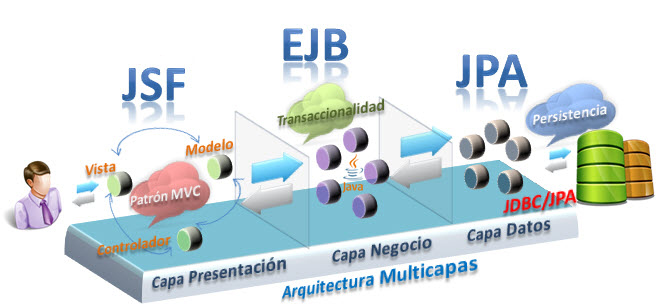
\includegraphics[width=0.75\textwidth]{img/arquitectura-jee.jpg}
    \end{center}
      \caption{Arquitectura multicapas con frameworks}
    \label{fig:arquitectura-jee}
  \end{figure}
\end{frame}


\begin{frame}{Estructura de Ficheros}
  \begin{columns}[onlytextwidth]
    \begin{column}{0.5\textwidth}
      \centering
      \begin{figure}[H]
        \begin{center}
        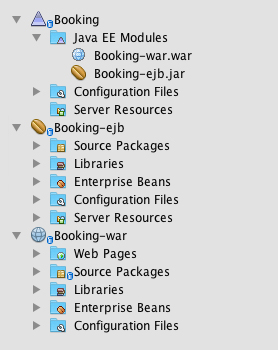
\includegraphics[width=0.7\textwidth]{img/estructura-ficheros.jpg}
        \end{center}
        \caption{Estructura de ficheros}
        \label{fig:estructura-proyecto}
      \end{figure}
    \end{column}
    \begin{column}{0.5\textwidth}
    \end{column}
€‹  \end{columns}
\end{frame}

\begin{frame}{Estructura de Ficheros}
  \begin{columns}[onlytextwidth]
    \begin{column}{0.5\textwidth}
      \centering
      \begin{figure}[H]
        \begin{center}
        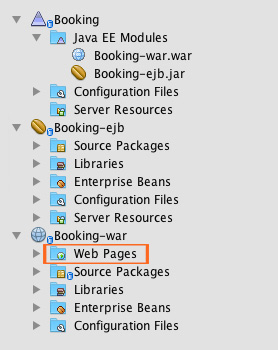
\includegraphics[width=0.7\textwidth]{img/estructura-ficheros-web.jpg}
        \end{center}
        \caption{Estructura de ficheros}
        \label{fig:estructura-proyecto}
      \end{figure}
    \end{column}
    \begin{column}{0.5\textwidth}
      \centering
      \begin{figure}[H]
        \begin{center}
        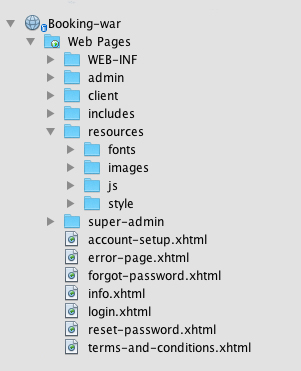
\includegraphics[width=0.7\textwidth]{img/web-pages.jpg}
        \end{center}
        \caption{Directorio Web Pages}
        \label{fig:estructura-web}
      \end{figure}
    \end{column}
€‹  \end{columns}
\end{frame}


\begin{frame}{web.xml}
  \begin{figure}[H]
    \begin{center}
        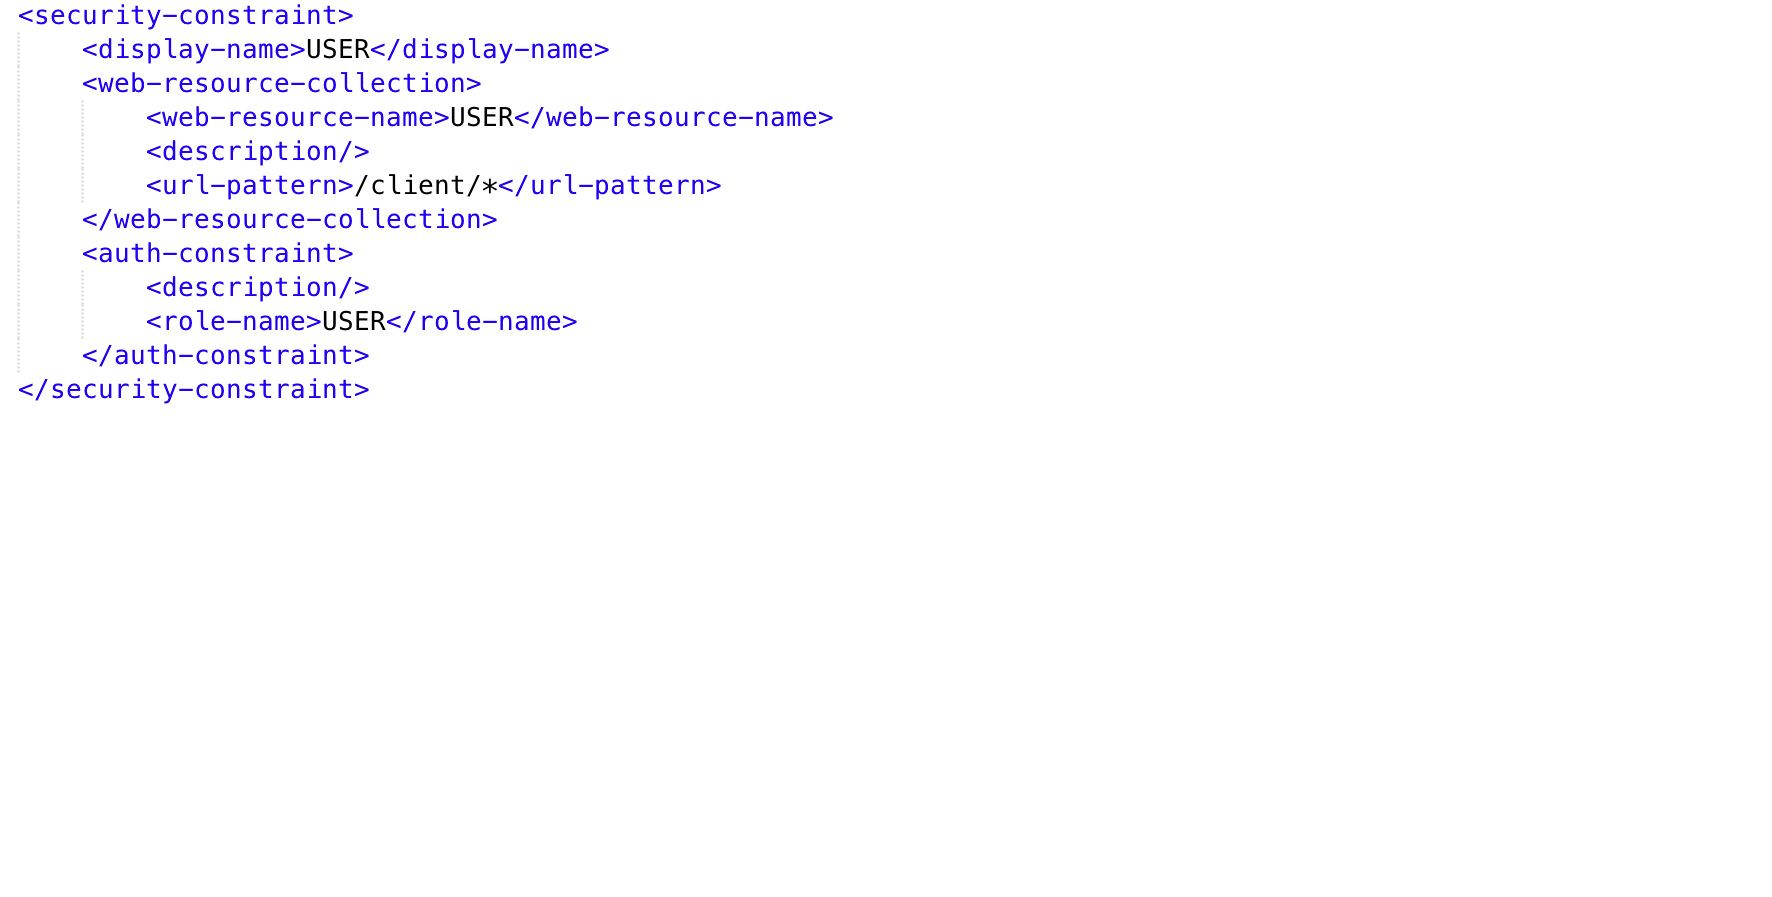
\includegraphics[width=\textwidth]{img/web-xml-client.jpg}
    \end{center}
    \label{fig:web-xml-client}
  \end{figure}
\end{frame}

\begin{frame}{web.xml}
  \begin{figure}[H]
    \begin{center}
        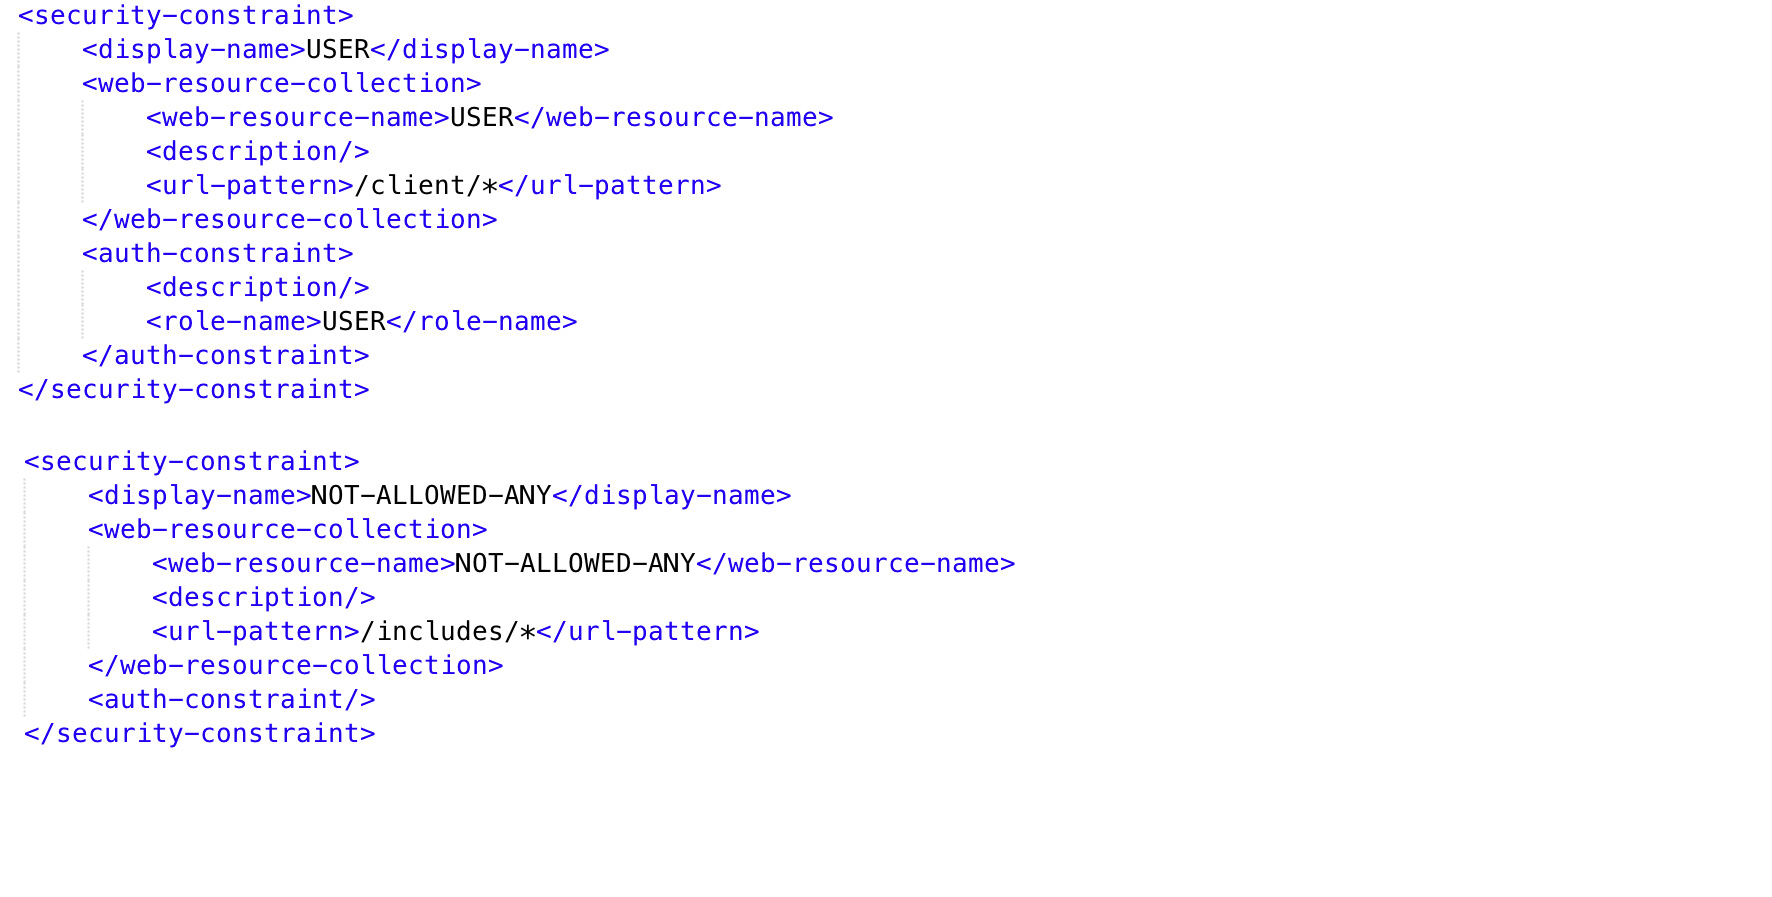
\includegraphics[width=\textwidth]{img/web-xml-includes.jpg}
    \end{center}
    \label{fig:web-xml-includes}
  \end{figure}
\end{frame}

\begin{frame}{web.xml}
  \begin{figure}[H]
    \begin{center}
        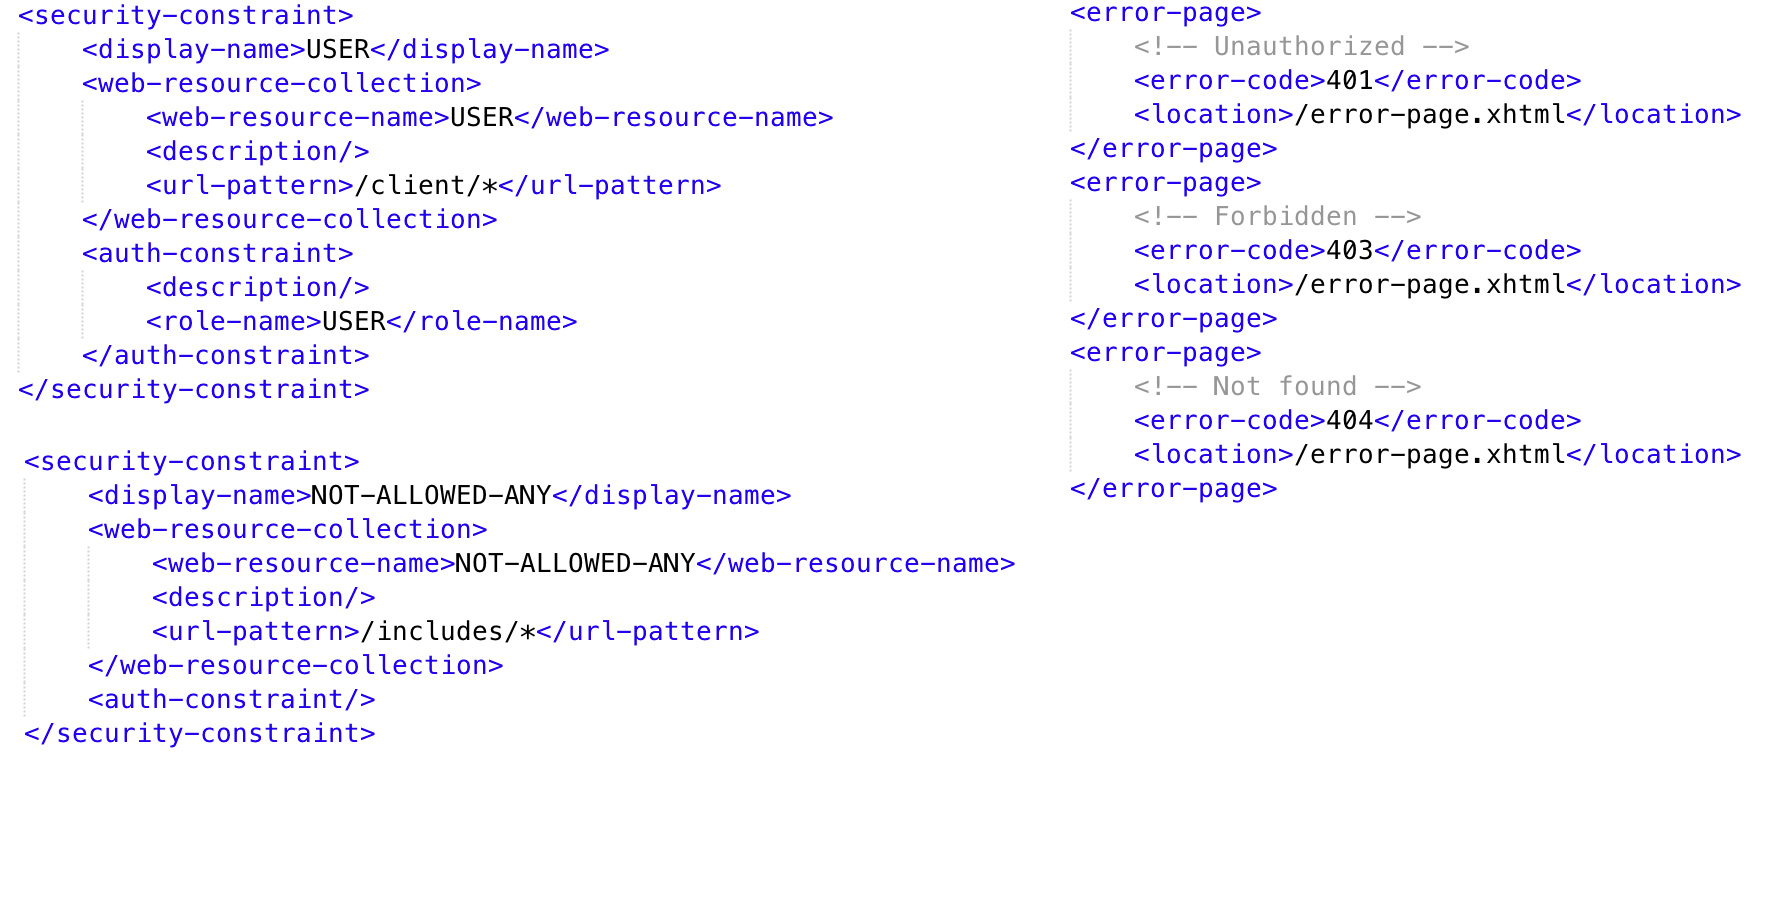
\includegraphics[width=\textwidth]{img/web-xml-errores.jpg}
    \end{center}
    \label{fig:web-xml-errores}
  \end{figure}
\end{frame}

\begin{frame}{web.xml}
  \begin{figure}[H]
    \begin{center}
        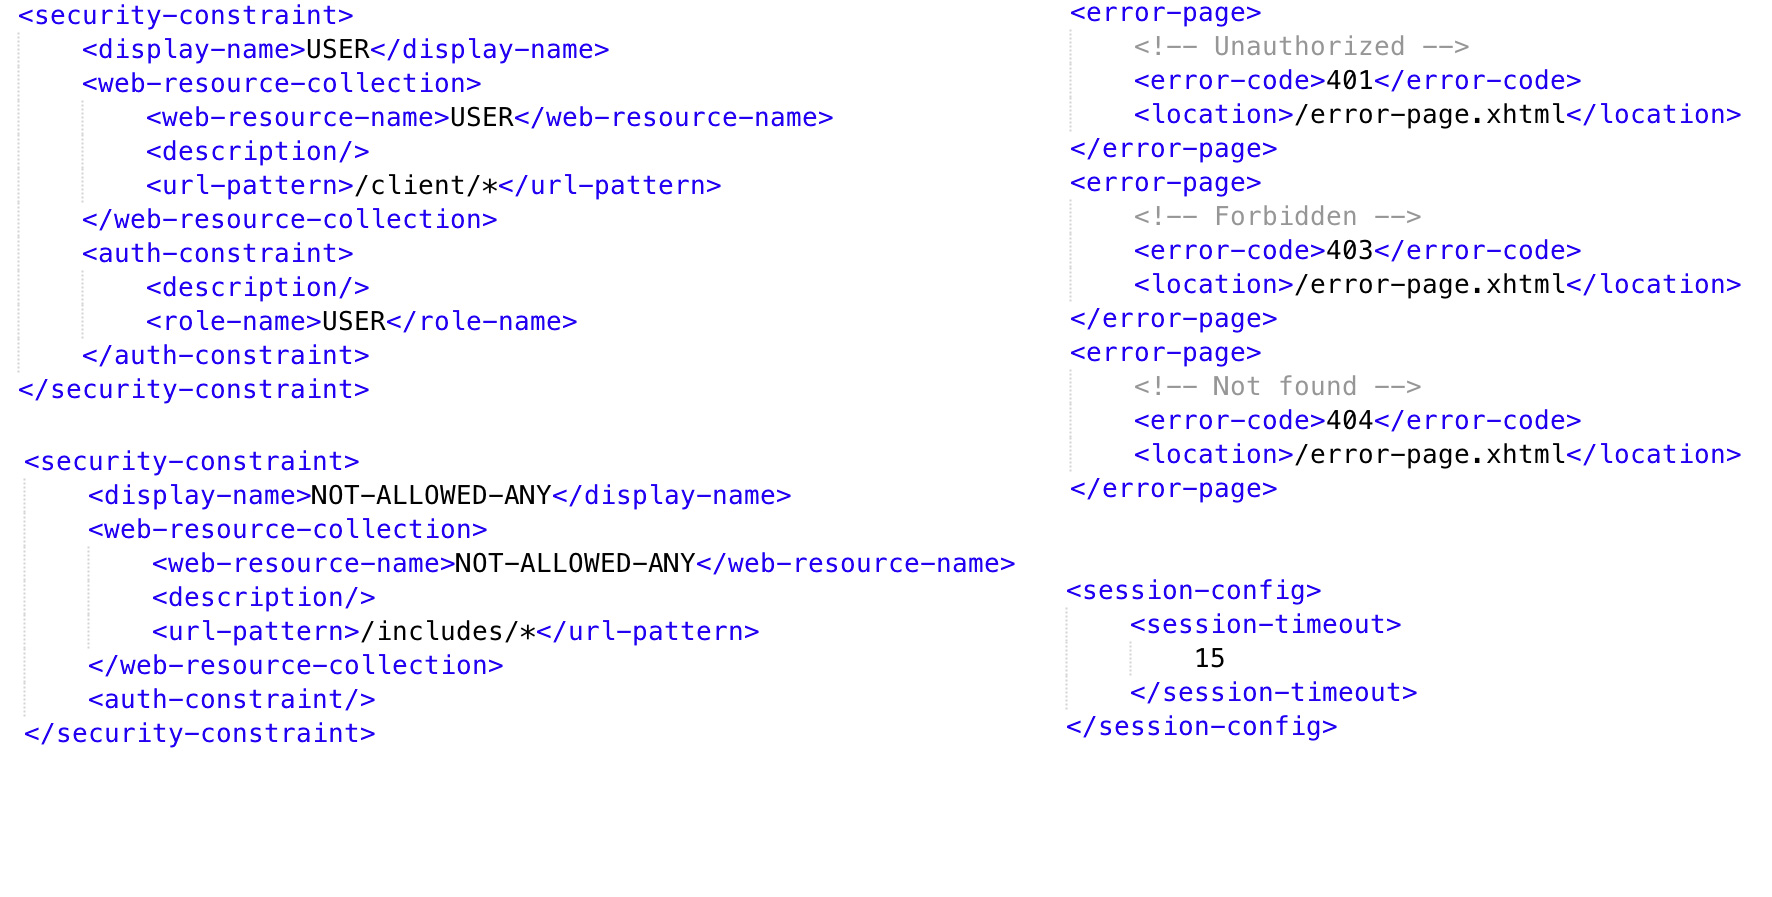
\includegraphics[width=\textwidth]{img/web-xml-sesion.jpg}
    \end{center}
    \label{fig:web-xml-sesion}
  \end{figure}
\end{frame}

\begin{frame}{web.xml}
  \begin{figure}[H]
    \begin{center}
        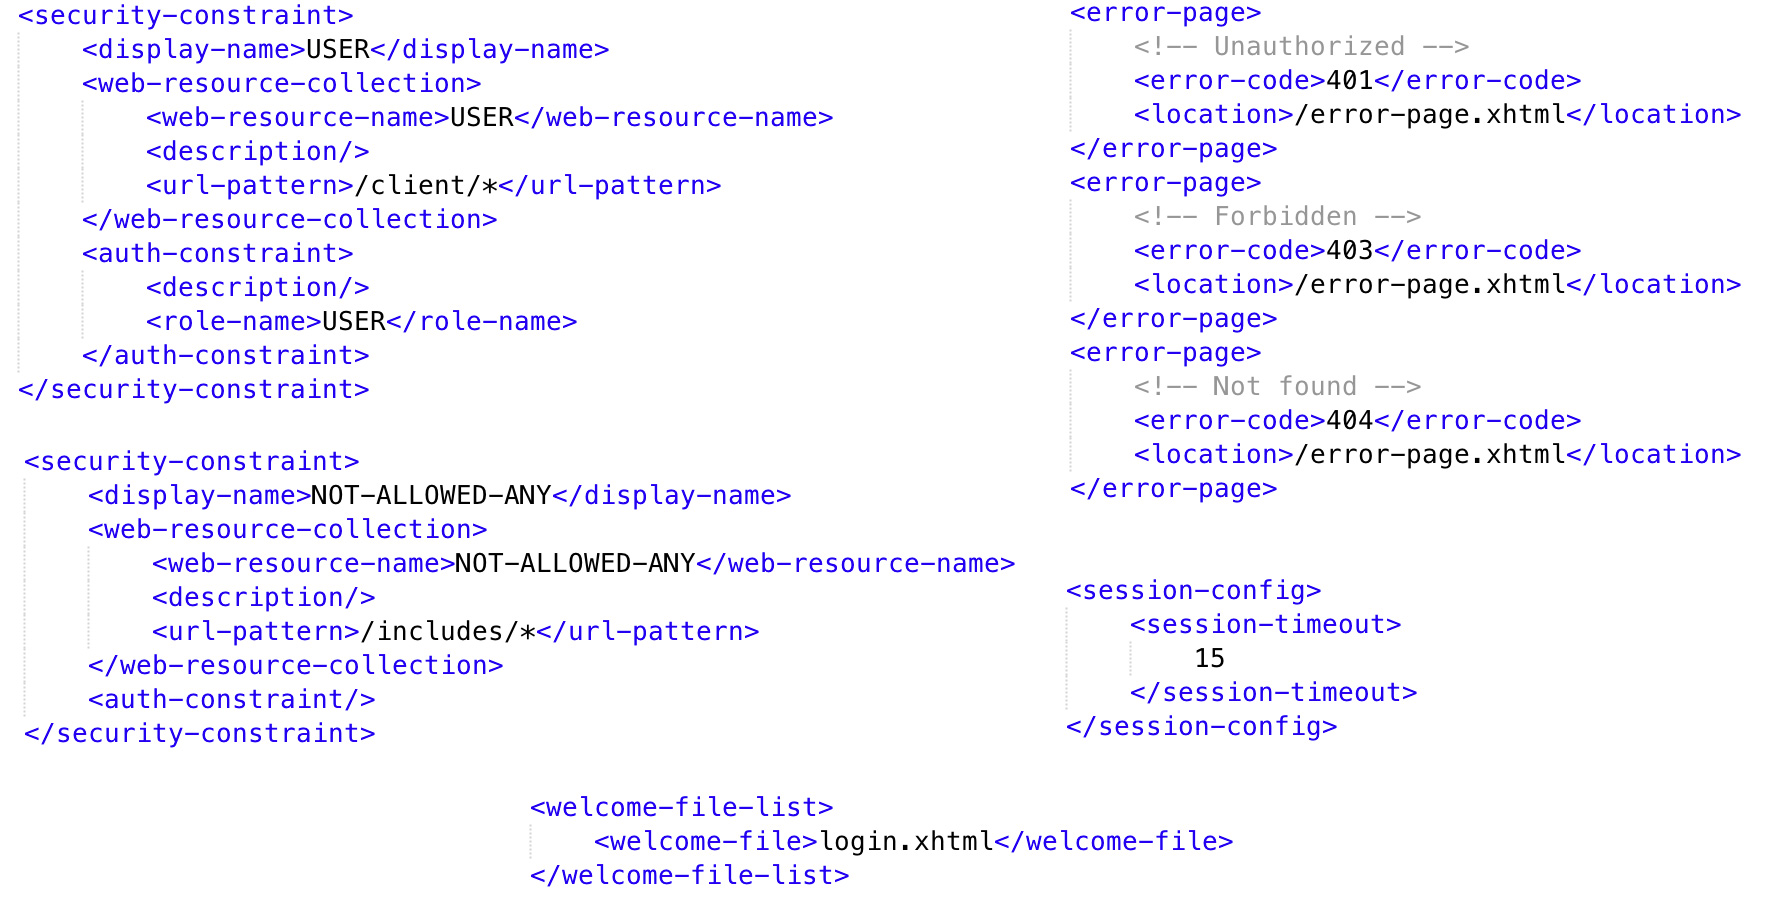
\includegraphics[width=\textwidth]{img/web-xml-login.jpg}
    \end{center}
    \label{fig:web-xml-login}
  \end{figure}
\end{frame}


\begin{frame}{Estructura de Ficheros}
  \begin{columns}[onlytextwidth]
    \begin{column}{0.5\textwidth}
      \centering
      \begin{figure}[H]
        \begin{center}
        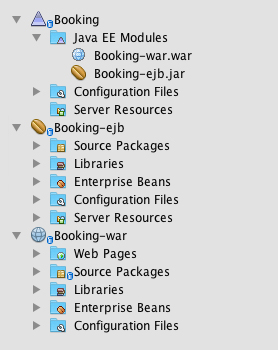
\includegraphics[width=0.7\textwidth]{img/estructura-ficheros.jpg}
        \end{center}
        \caption{Estructura de ficheros}
        \label{fig:estructura-proyecto-3}
      \end{figure}
    \end{column}
    \begin{column}{0.5\textwidth}
    \end{column}
€‹  \end{columns}
\end{frame}

\begin{frame}{Estructura de Ficheros}
  \begin{columns}[onlytextwidth]
    \begin{column}{0.5\textwidth}
      \centering
      \begin{figure}[H]
        \begin{center}
        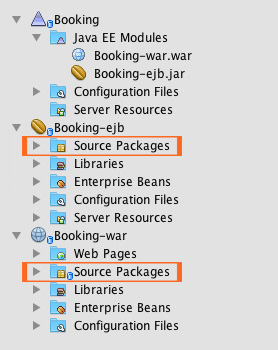
\includegraphics[width=0.7\textwidth]{img/estructura-ficheros-war-ejb-sources.jpg}
        \end{center}
        \caption{Estructura de ficheros}
        \label{fig:estructura-proyecto-4}
      \end{figure}
    \end{column}
    \begin{column}{0.5\textwidth}
      \centering
      \begin{figure}[H]
        \begin{center}
        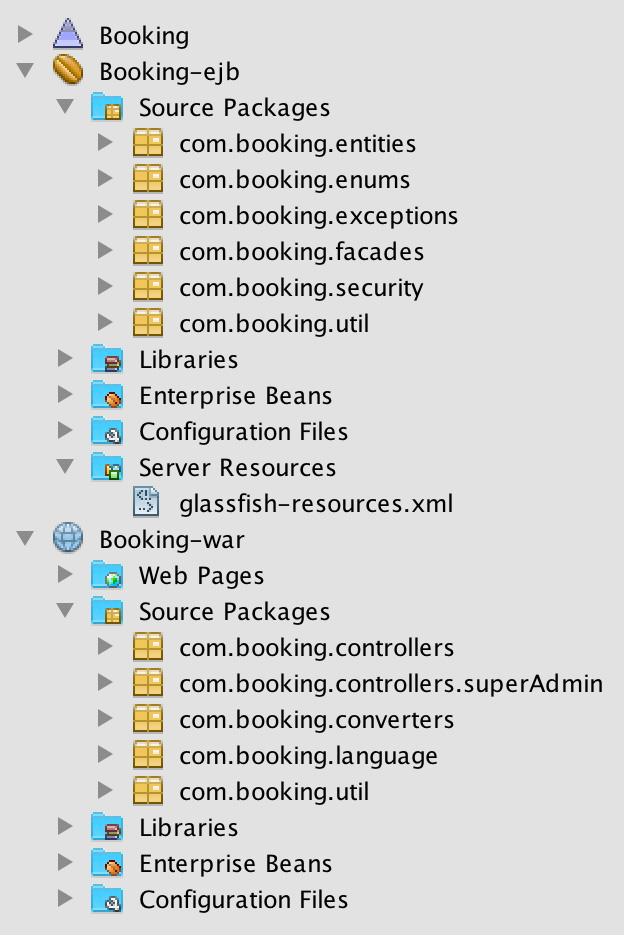
\includegraphics[width=0.7\textwidth]{img/estructura-ficheros-war-ejb-sources-abierto.jpg}
        \end{center}
        \label{fig:estructura-web}
      \end{figure}
    \end{column}
€‹  \end{columns}
\end{frame}


\begin{frame}{Comunicación por Capas}
  \begin{figure}[H]
    \begin{center}
        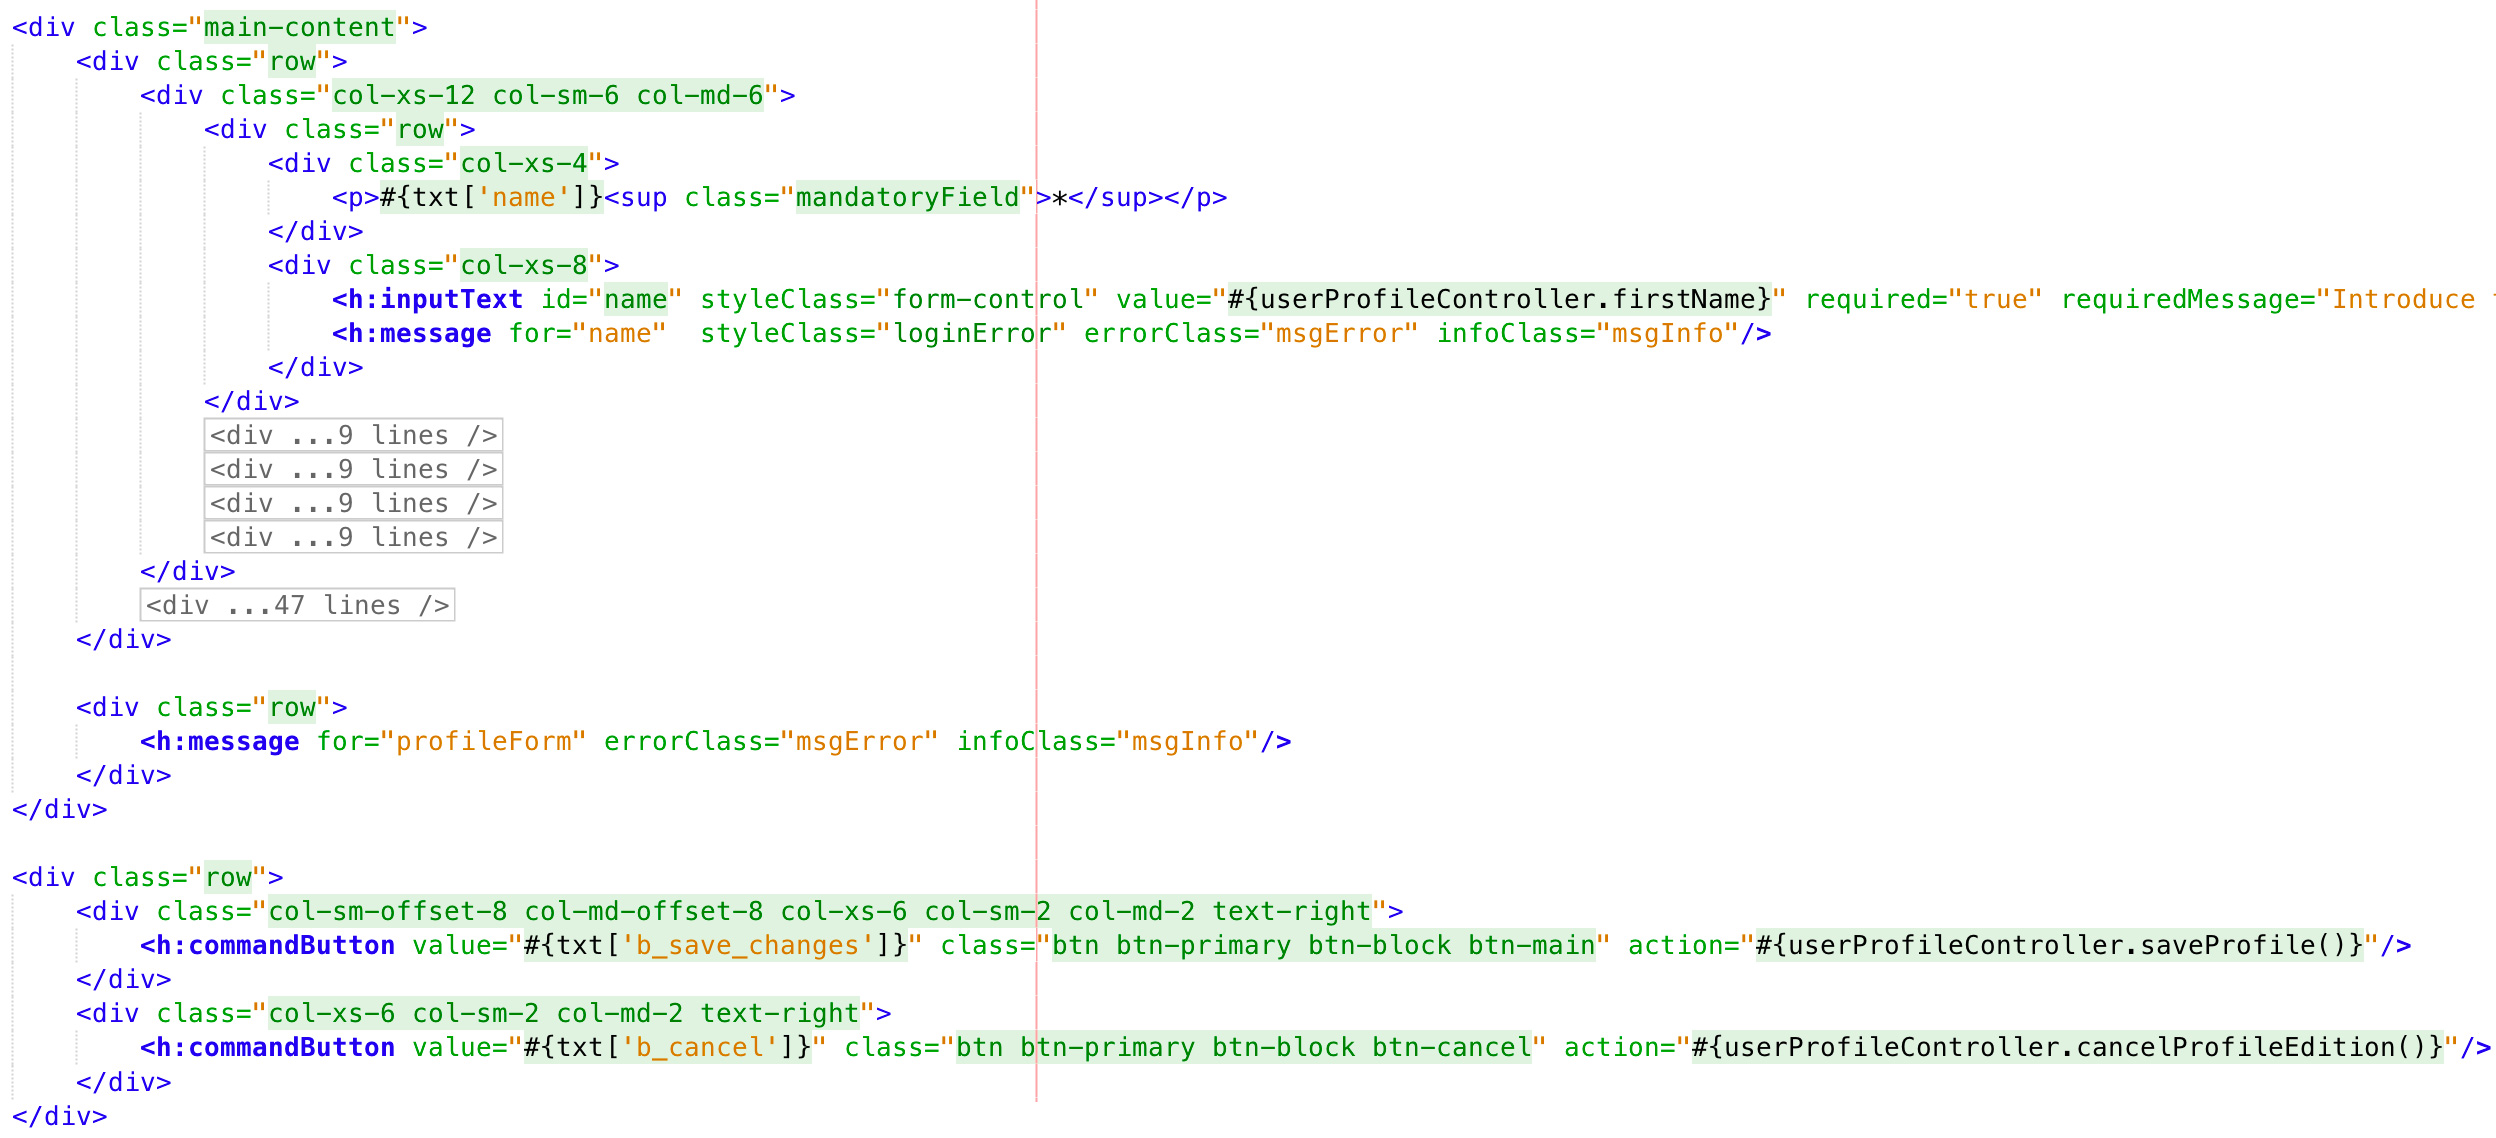
\includegraphics[width=\textwidth]{img/ejemplo-jsf.jpg}
    \end{center}
    \label{fig:ejemplo-jsf}
  \end{figure}
\end{frame}

\begin{frame}{Comunicación por Capas}
  \begin{figure}[H]
    \begin{center}
        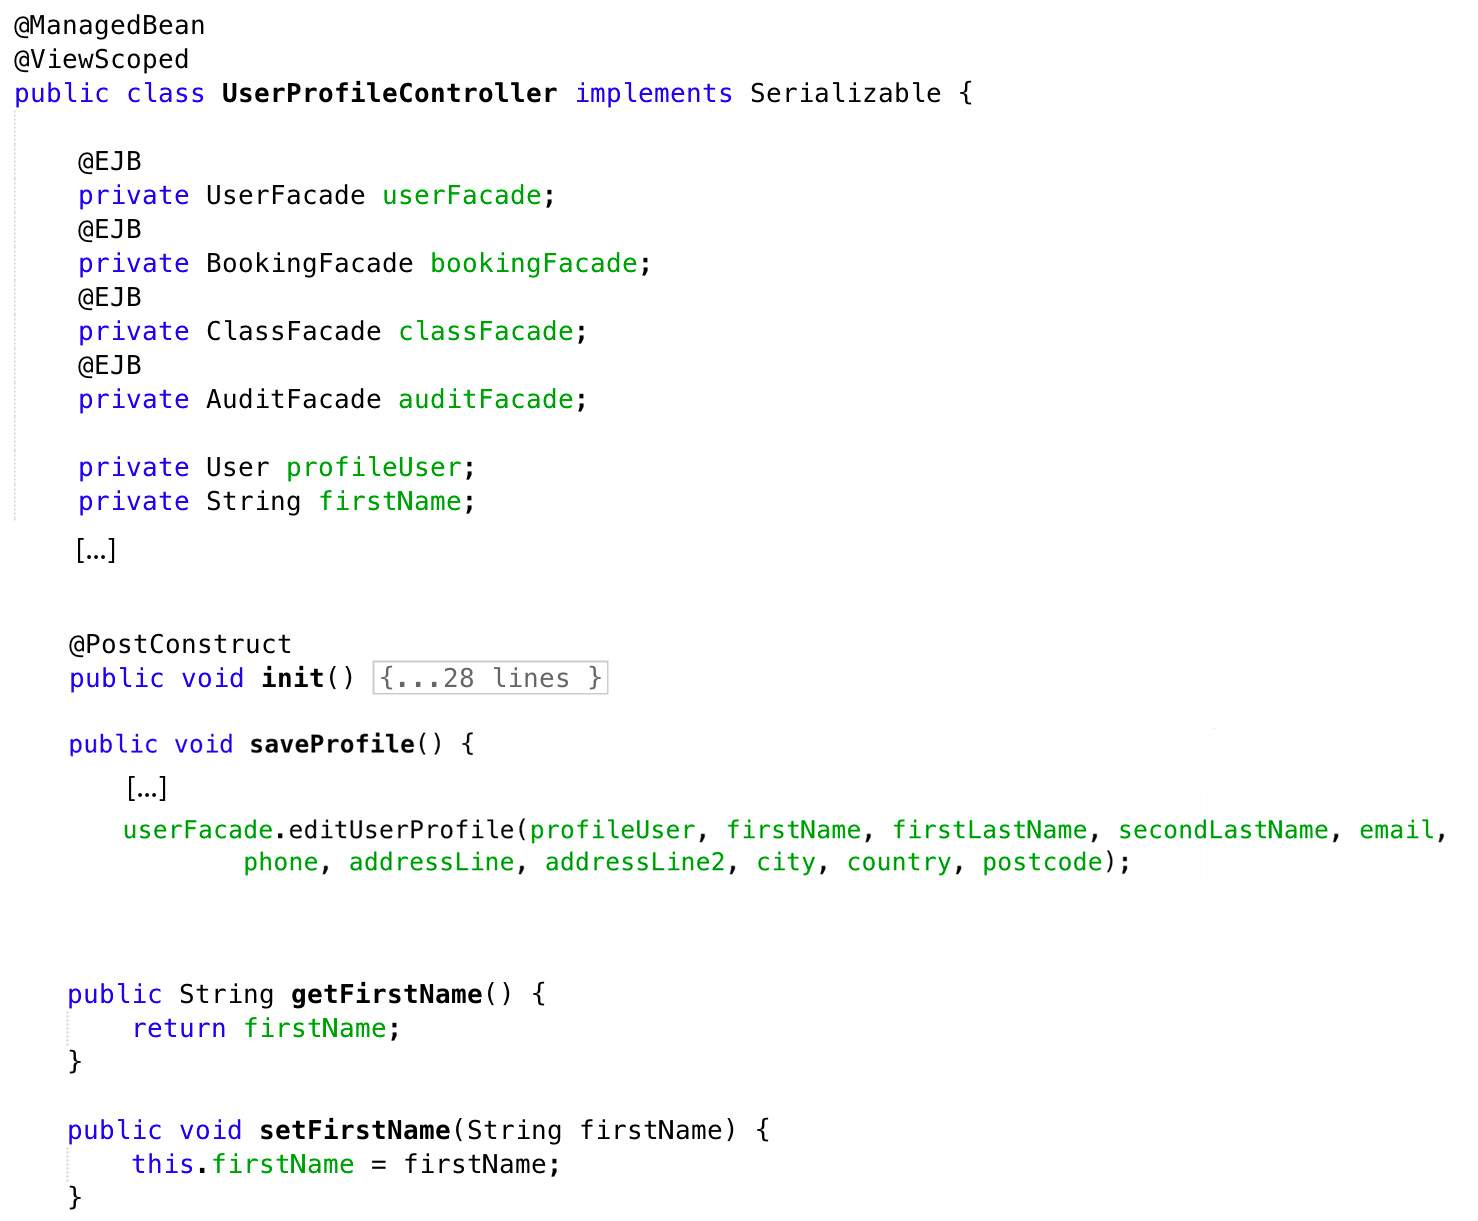
\includegraphics[width=0.7\textwidth]{img/ejemplo-controlador.jpg}
    \end{center}
    \label{fig:ejemplo-ejb}
  \end{figure}
\end{frame}

\begin{frame}{Comunicación por Capas}
  \begin{figure}[H]
    \begin{center}
        \includegraphics[width=0.75\textwidth]{img/comunicacion-capas.png}
    \end{center}
    \label{fig:comunicacion-capas}
  \end{figure}
\end{frame}


\begin{frame}{Pruebas}
  \begin{block}{Niveles de Pruebas}
    \begin{itemize}
      \item Pruebas unitarias.
      \item Pruebas de integración.
      \item Pruebas de sistema:
      \begin{itemize}
        \item Pruebas funcionales.
        \item Pruebas no funcionales.
      \end{itemize}
  \end{itemize}
  \end{block}
\end{frame}



%%%%%%%%%%%%%%%%%%%%%%%%%%%%%%%
\section{Demostración}
\begin{frame}{Demostración}
  \tableofcontents[currentsection]
\end{frame}

\begin{frame}{Demostración}
  \begin{center}
    \Huge{DEMOSTRACIӓN}
  \end{center}
\end{frame}


%%%%%%%%%%%%%%%%%%%%%%%%%%%%%%%
\section{Conclusiones}
\frame{\frametitle{Conclusiones}\tableofcontents[currentsection]}

\subsection*{Objetivos alcanzados}
\begin{frame}{Objetivos alcanzados}
\begin{block}{Los objetivos alcanzados han sido...}
  \begin{itemize}
    \item La aplicación es capáz de resolver y almacenar los modelos de los
      proyectos Django.
    \item Gestionar vocabularios y configuración de modelos.
    \item Herramientas para la publicación de datos.
    \item Se han cumplido los plazos.
  \end{itemize}
\end{block}
\end{frame}

\subsection*{Lecciones aprendidas}
\begin{frame}{Lecciones aprendidas}
\begin{block}{Valoración...}
  \begin{itemize}
    \item Se han adquirido mejores conocimientos tanto del lenguaje Python como
      del framework Django.
    \item Importancia de seguir una metodologí­a de trabajo, realizar una
      planificación del proyecto y un análisis y diseño del mismo.
    \item Se han adquirido nuevos conceptos relacionados con la Web Semántica.
    \item Trabajado con nuevas tecnologí­as y herramientas como SPARQL, RDF o
      D2Rq.
    \item Se han adquirido buenas prácticas a la hora de programar en
      Python/Django.
  \end{itemize}
\end{block}
\end{frame}

\subsection*{Trabajo futuro}
\begin{frame}{Trabajo futuro}
\begin{block}{Trabajos futuros...}
El trabajo futuro en esta aplicación podrí­a abarcarse desde diferentes frentes:
\begin{itemize}
\item Varias configuraciones simultáneas.
\item Consulta sobre la base de datos haciendo uso de SPARQL.
\item Ampliar formatos de exportación de datos.
\item Ampliar la disponibilidad a otros frameworks.
\end{itemize}
\end{block}
\end{frame}

\section{Bibliografí­a}
\begin{frame}{Bibliografí­a}
  \tableofcontents[currentsection]
\end{frame}

\begin{frame}{Bibliografí­a}
  \begin{thebibliography}{10}
    \beamertemplatebookbibitems
    \bibitem{12} DjangoFoundation. \emph{Web oficial del proyecto Django, https://www.djangoproject.com/}. 2013.
    \bibitem{20} Documentación oficial Python, http://www.python.org/, 2013.
    \bibitem{13} Bob DuCharme, Learning sparql, O'€™Reilly, 2011.
    \bibitem{14} Tom Heath and Christian Bizer, LinkedDataBook, http://linkeddatabook.com/editions/1.0/, 2011.
    \bibitem{21} Guido Van Rossum and Barry Warsaw, Style Guide for Python Code, http://www.python.org/dev/peps/pep-0008/, 2012.
    \bibitem{15} jQuery, Documentación oficial jQuery, http://api.jquery.com/, 2013.
    \bibitem{16} Twitter, Bootstrap V3, http://getbootstrap.com/, 2013.
    %\bibitem{bibliografia1}....
  \end{thebibliography} 
\end{frame}

\begin{frame}{Bibliografí­a}
  \begin{thebibliography}{10}
    \beamertemplatebookbibitems
    \bibitem{17} Documentación oficial D2Rq, http://d2rq.org/, 2013.
    \bibitem{18} Project FOAF, FOAF, http://www.foaf-project.org/, 2010.
    \bibitem{19} Google-Microsoft-Yahoo!, Schema, http://schema.org/, 2012.
    \bibitem{22} Martin Hepp, Good Relations, http://www.heppnetz.de/projects/goodrelations/, 2012.
    \bibitem{24} W3C OWL, OWL, http://www.w3.org/TR/owl-ref/, 2004.
    \bibitem{24} W3C Microdata, Microdata, http://www.w3.org/TR/microdata/, 2013.
    \bibitem{27} W3C RDF, RDF, http://www.w3.org/TR/rdf-primer/, 2004.
    %\bibitem{bibliografia1}....
  \end{thebibliography} 
\end{frame}

\begin{frame}{Bibliografí­a}
  \begin{thebibliography}{10}
    \beamertemplatebookbibitems
    \bibitem{28} W3C RDFa, RDFa, http://www.w3.org/TR/rdfa-syntax/, 2013.
    \bibitem{25} W3C RDFS, RDFS, http://www.w3.org/TR/rdf-schema/, 2004.
    \bibitem{26} Ministerio de Hacienda y Administraciones Públicas de España, MAGERIT V3, 2012.
    \bibitem{23} Infojobs, Salarios Infojobs, http://plandecarrera.infojobs.net/, 2013.
    %\bibitem{bibliografia1}....
  \end{thebibliography} 
\end{frame}


\appendix
\frame
{
  \begin{center}
    \Huge{Gracias por su atención}
  \end{center}
  \begin{center}
    \url{https://pypi.python.org/pypi/django-easydata/}
  \end{center}
}
\end{document}
